The trigger strategy for the analysis in Run-2 is similar to the one used in the Run-1 version. There, a combination of \met , 
single-lepton and di-lepton triggers was used for the selection of events in the signal region and control distributions. The triggers were checked consecutively starting with the \met\ trigger, followed by the single lepton trigger and the dilepton triggers, until one of the triggers is passed by the event. Offline cuts on the missing energy and the \pt\ of the triggered objects were applied to ensure to be on the efficiency \textit{plateau} of the corresponding trigger.

For Run-2 the triggers to be used are also missing energy and single- and di-lepton triggers. The lepton trigger menu includes triggers selecting isolated and non-isolated leptons as well as dilepton triggers selecting mixed-flavor lepton events. 
The following triggers have been regarded as important for this analysis and were used for further studies on performance and efficiency:

\begin{itemize}
\item Single-lepton triggers: \texttt{HLT\_mu26, HLT\_mu50, HLT\_mu24\_imedium, HLT\_mu26\_imedium}, 

\texttt{HLT\_e20\_medium, HLT\_e60\_medium, HLT\_e24\_tight\_iloose, HLT\_e26\_tight\_iloose}

\item Di-lepton triggers: \texttt{HLT\_2m10, HLT\_2mu14, HLT\_2e12\_loose\_L12EM10VH, HLT\_2e17\_loose, HLT\_e17\_loose\_mu14}

\item Multi-lepton triggers \texttt{HLT\_3m6, HLT\_e12\_loose\_2mu10}

\item \met\ triggers: \texttt{HLT\_xe60, HLT\_xe70, HLT\_xe100, HLT\_xe100\_cell}

\end{itemize}

The performance of these triggers has been investigated by running the analysis 
on dedicated $Z \rightarrow \mu \mu$, $Z \rightarrow ee$ and $t \bar{t}$ Monte 
Carlo samples with several trigger applications.
For each object triggered, an offline cut on the object \pt\ or the \met\ is applied to ensure the full efficiency of the trigger in the selected event. A geometrical $\Delta R$ matching between the lepton triggers fired and the signal leptons reconstructed in each event is applied in order to confirm that the according trigger was activated by one of the signal leptons found in the analysis. 


\subsubsection{Monte Carlo samples and software framework}

The trigger studies were performed with the latest available releases of the ATLAS software framework and the latest Monte Carlo productions. The analysis code was setup with the \texttt{AnalysisBase} framework (2.3.8 branch for rel.20 ATLAS software). The object selection was done by using the \texttt{SUSYTools-00-06-03} package which provides the current recommendations for selection of signal and baseline objetcs. 

The Monte Carlo samples used for these studies are validation samples produced with the 20.1.4.3 MC15 ATLAS software release (no pileup). 

\begin{itemize}

\item $t \bar{t}$ sample: 

\texttt{valid3.110401.PowhegPythia\_P2012\_ttbar\_nonallhad.recon.AOD.e3099\_s2578\_r6540}

\item $Z \rightarrow \mu \mu$ sample:  

\texttt{valid3.167826.Sherpa\_CT10\_ZmumuMassiveCBPt280\_500\_CVetoBVeto.recon.AOD.e3099\_s2578\_r6540}

\item $Z \rightarrow e e$ sample: 

\texttt{valid3.147406.PowhegPythia8\_AZNLO\_Zee.recon.AOD.e3099\_s2578\_r6540}

\end{itemize}

\subsubsection{Total event yields}

The total event yields for the test MC samples and different trigger configurations was measured. The yields are shown in Fig.~\ref{fig:events} for the $t \bar{t}$ Monte Carlo sample and for the $Z \rightarrow \mu \mu$, $Z \rightarrow ee$ samples respectively. The trigger performance is as expected: while for $Z \rightarrow \mu \mu$ Monte Carlo, the muon triggers select most of the events, for $Z \rightarrow ee$ the electron triggers do. For $t \bar{t}$ Monte Carlo, the muon- and electron triggers have similar selection rates, and most events are selected by applying \met\ triggers.

\begin{figure}[htb!]
\centering
\subfigure{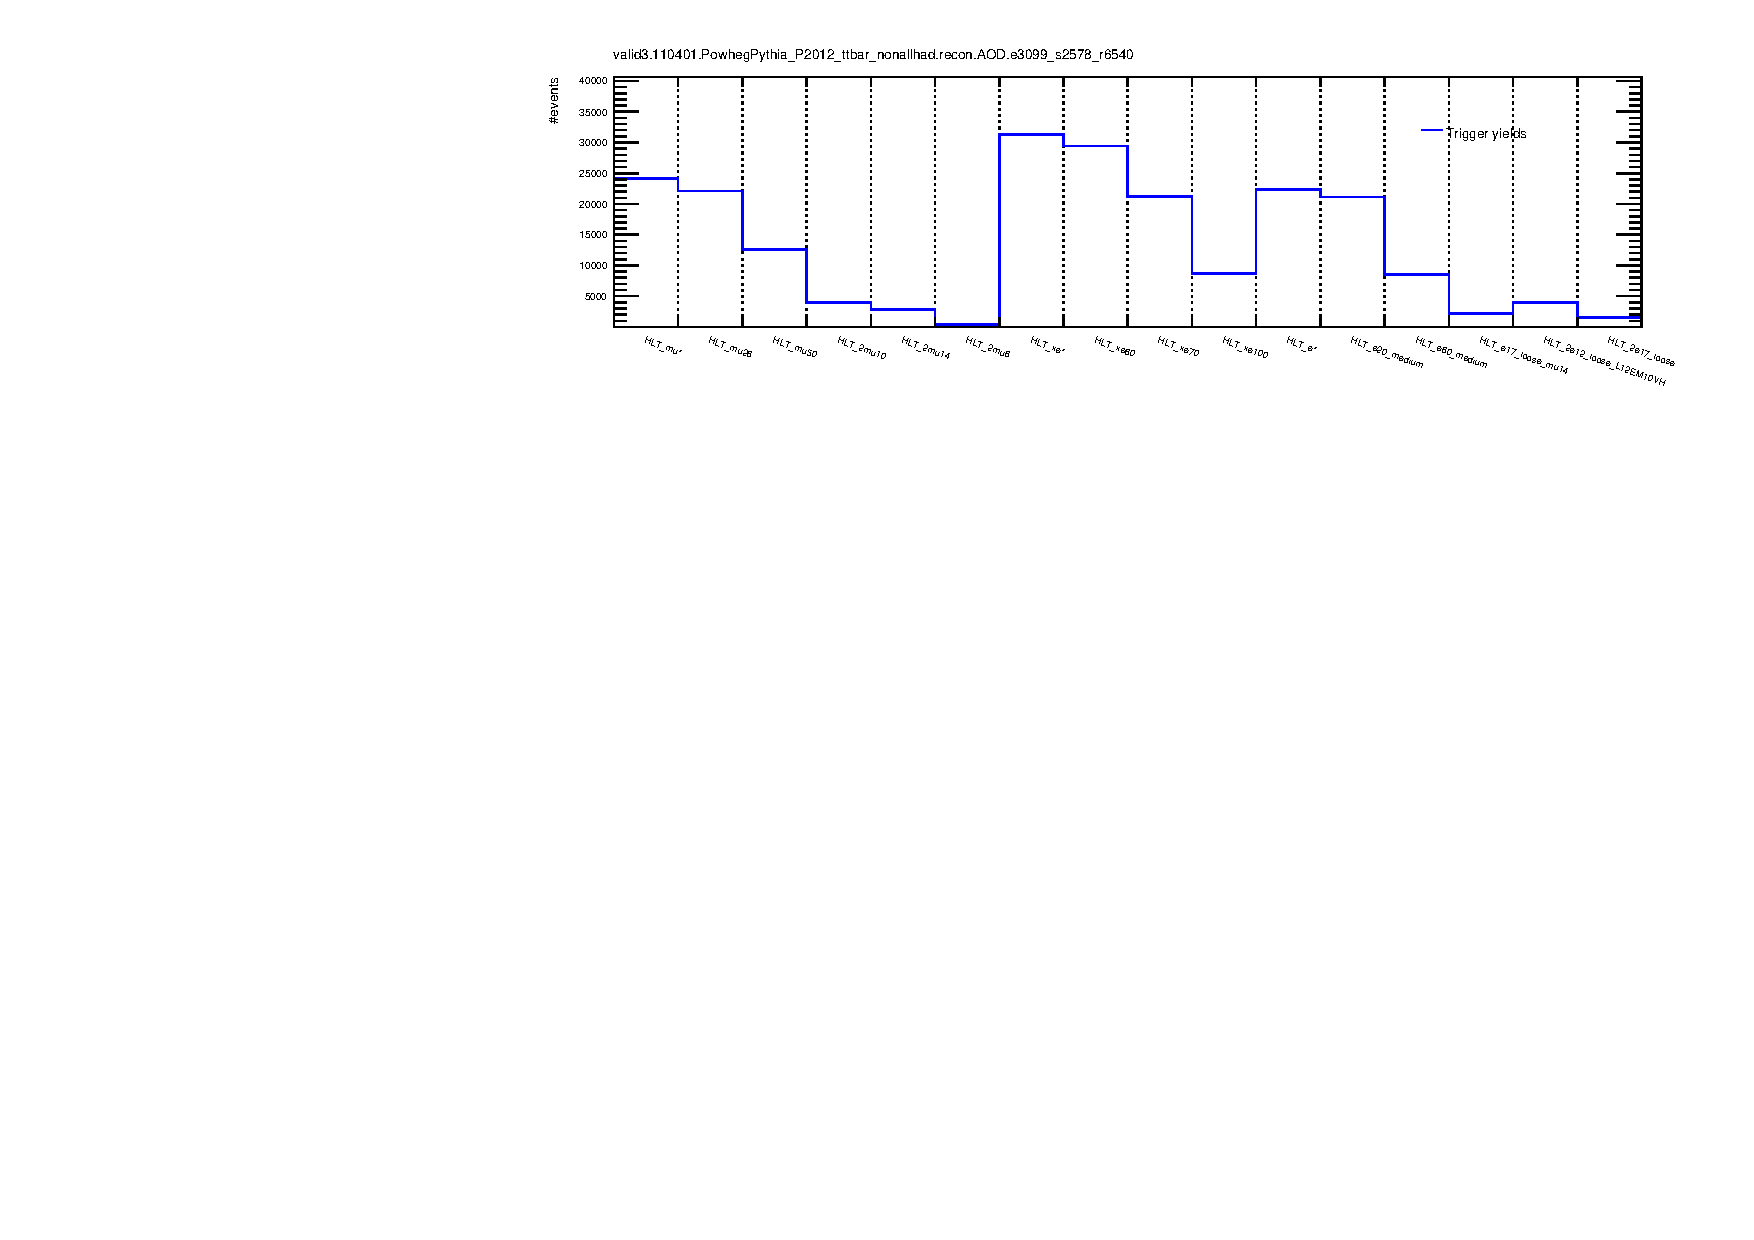
\includegraphics[width=1.\textwidth]{TRIGGER/Events_ttbar}}
\subfigure{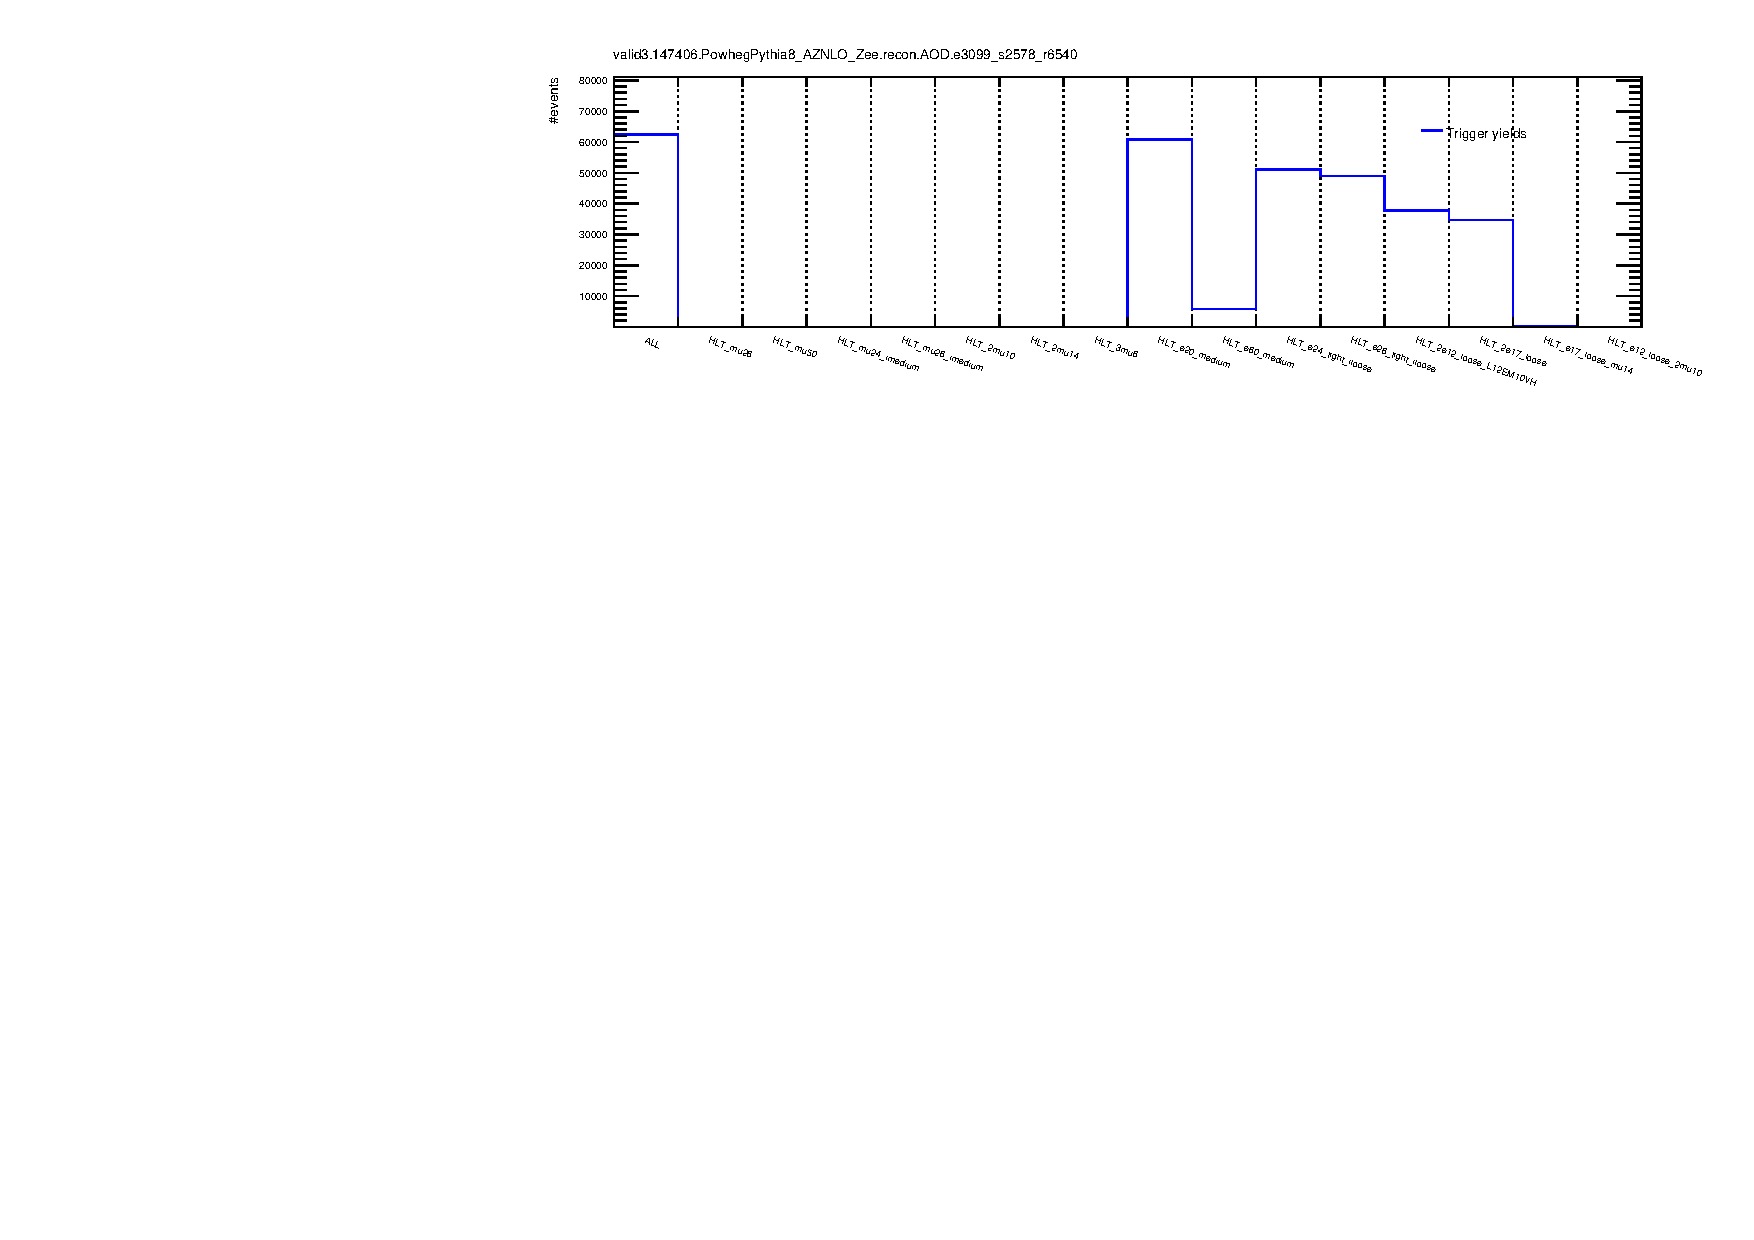
\includegraphics[width=1.\textwidth]{TRIGGER/Events_Zee}}
\subfigure{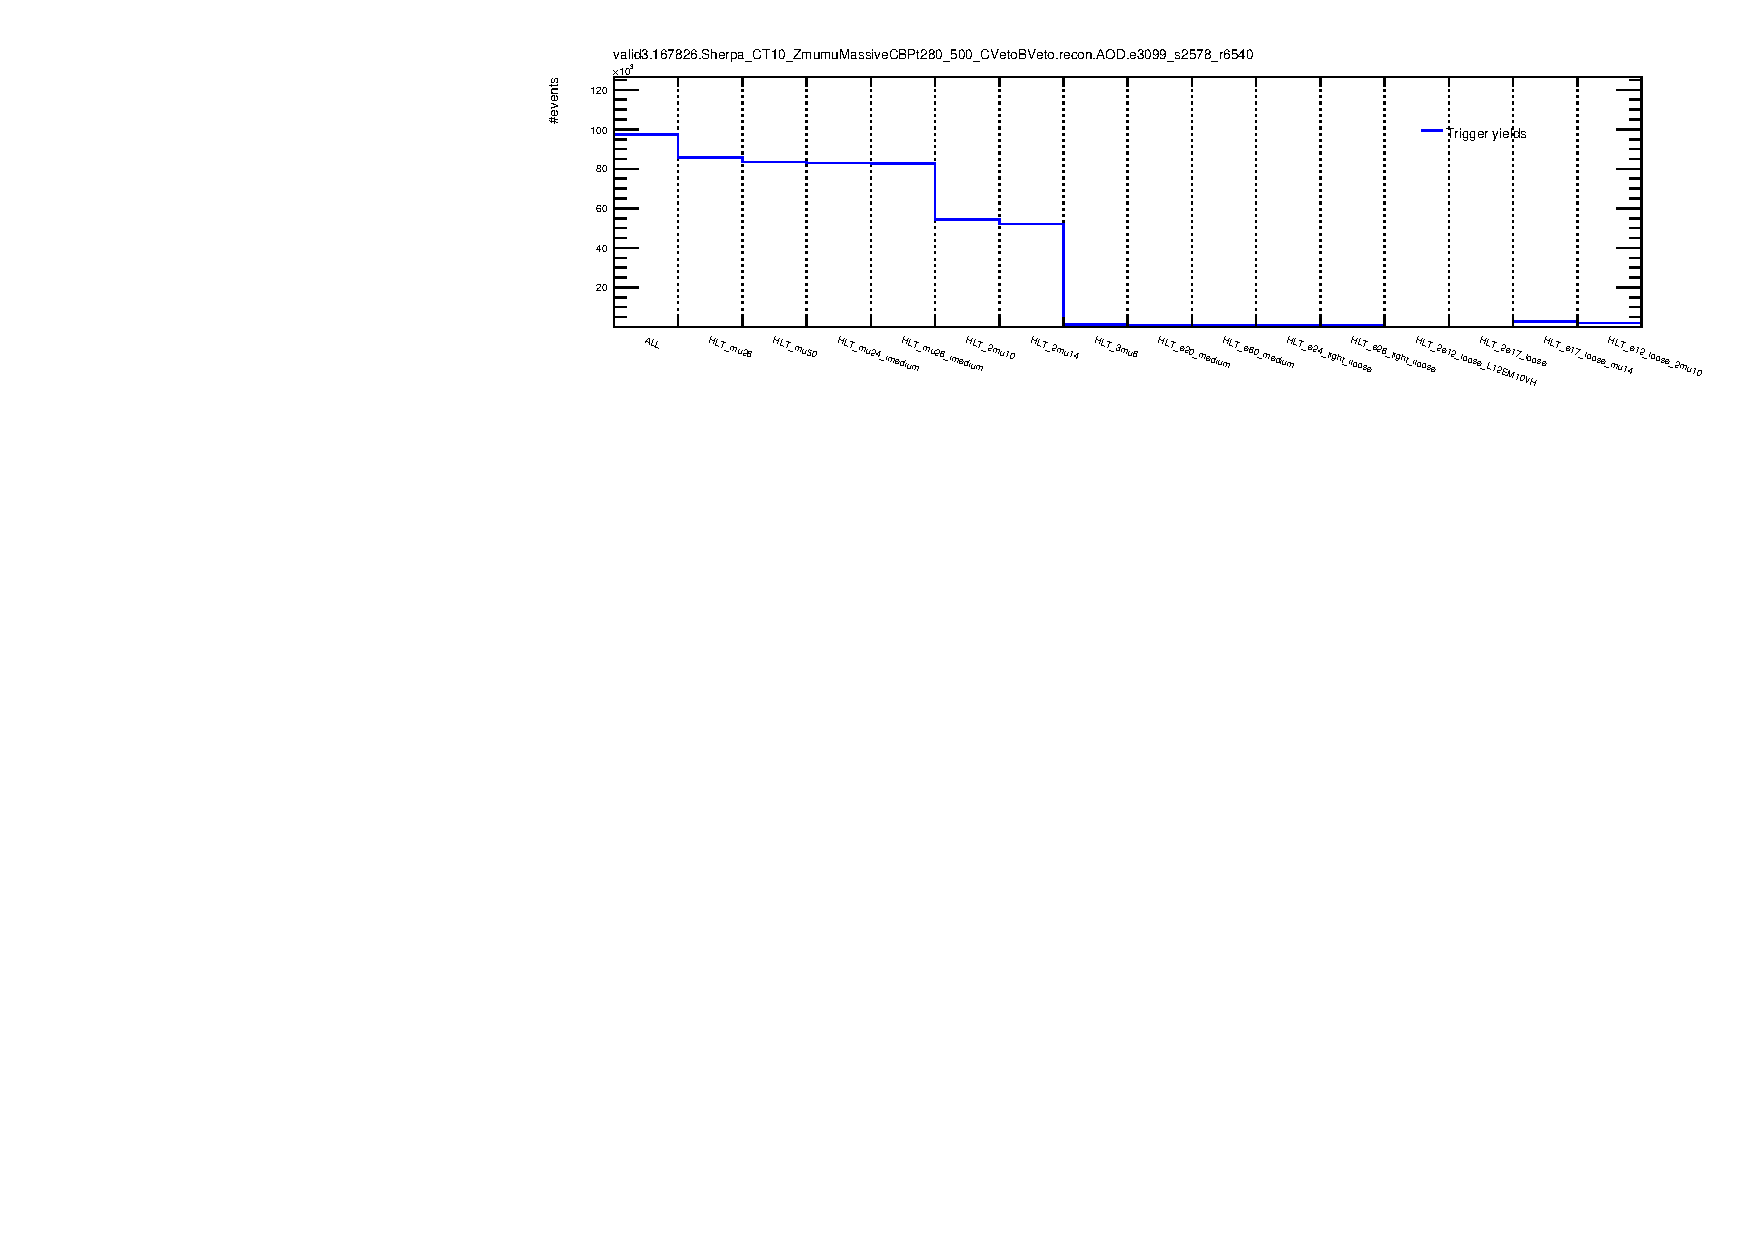
\includegraphics[width=1.\textwidth]{TRIGGER/Events_Zmumu}}
\caption{Total event yields for the $t \bar{t}$ sample (top) and for the $Z \rightarrow \mu \mu$ (middle), $Z \rightarrow ee$ (bottom) samples. On the x-axis the different triggers (or trigger configurations) are shown.}
\label{fig:events}
\end{figure}

\subsubsection{Efficiencies}

The trigger efficiency in Monte Carlo can be obtained by dividing the number of triggered events by the total number of events. The efficiencies have been calculated separately for single-lepton, dilepton triggers and for \met\ triggers. The results for some examples are shown in Fig.~\ref{fig:eff_singlelepton} for single lepton triggers and for dilepton and \met\ triggers on Fig.~\ref{fig:eff_dilepton_met}. Further efficiency plots can be found in Appendix~\ref{app_trigger}. The turn-on curves for the single-lepton and dilepton triggers show the expected evolution. The efficiency at the trigger plateau is between 95\% - 98\% for single-lepton and around 90\% for dilepton triggers. For the \met\ trigger, the turn-on is slower with respect to the quoted online threshold. It reaches its efficiency plateau if \met\ $>$ 250 GeV and the efficiency value in plateau is around 80\%.  

\begin{figure}[htb!]
\centering
\subfigure{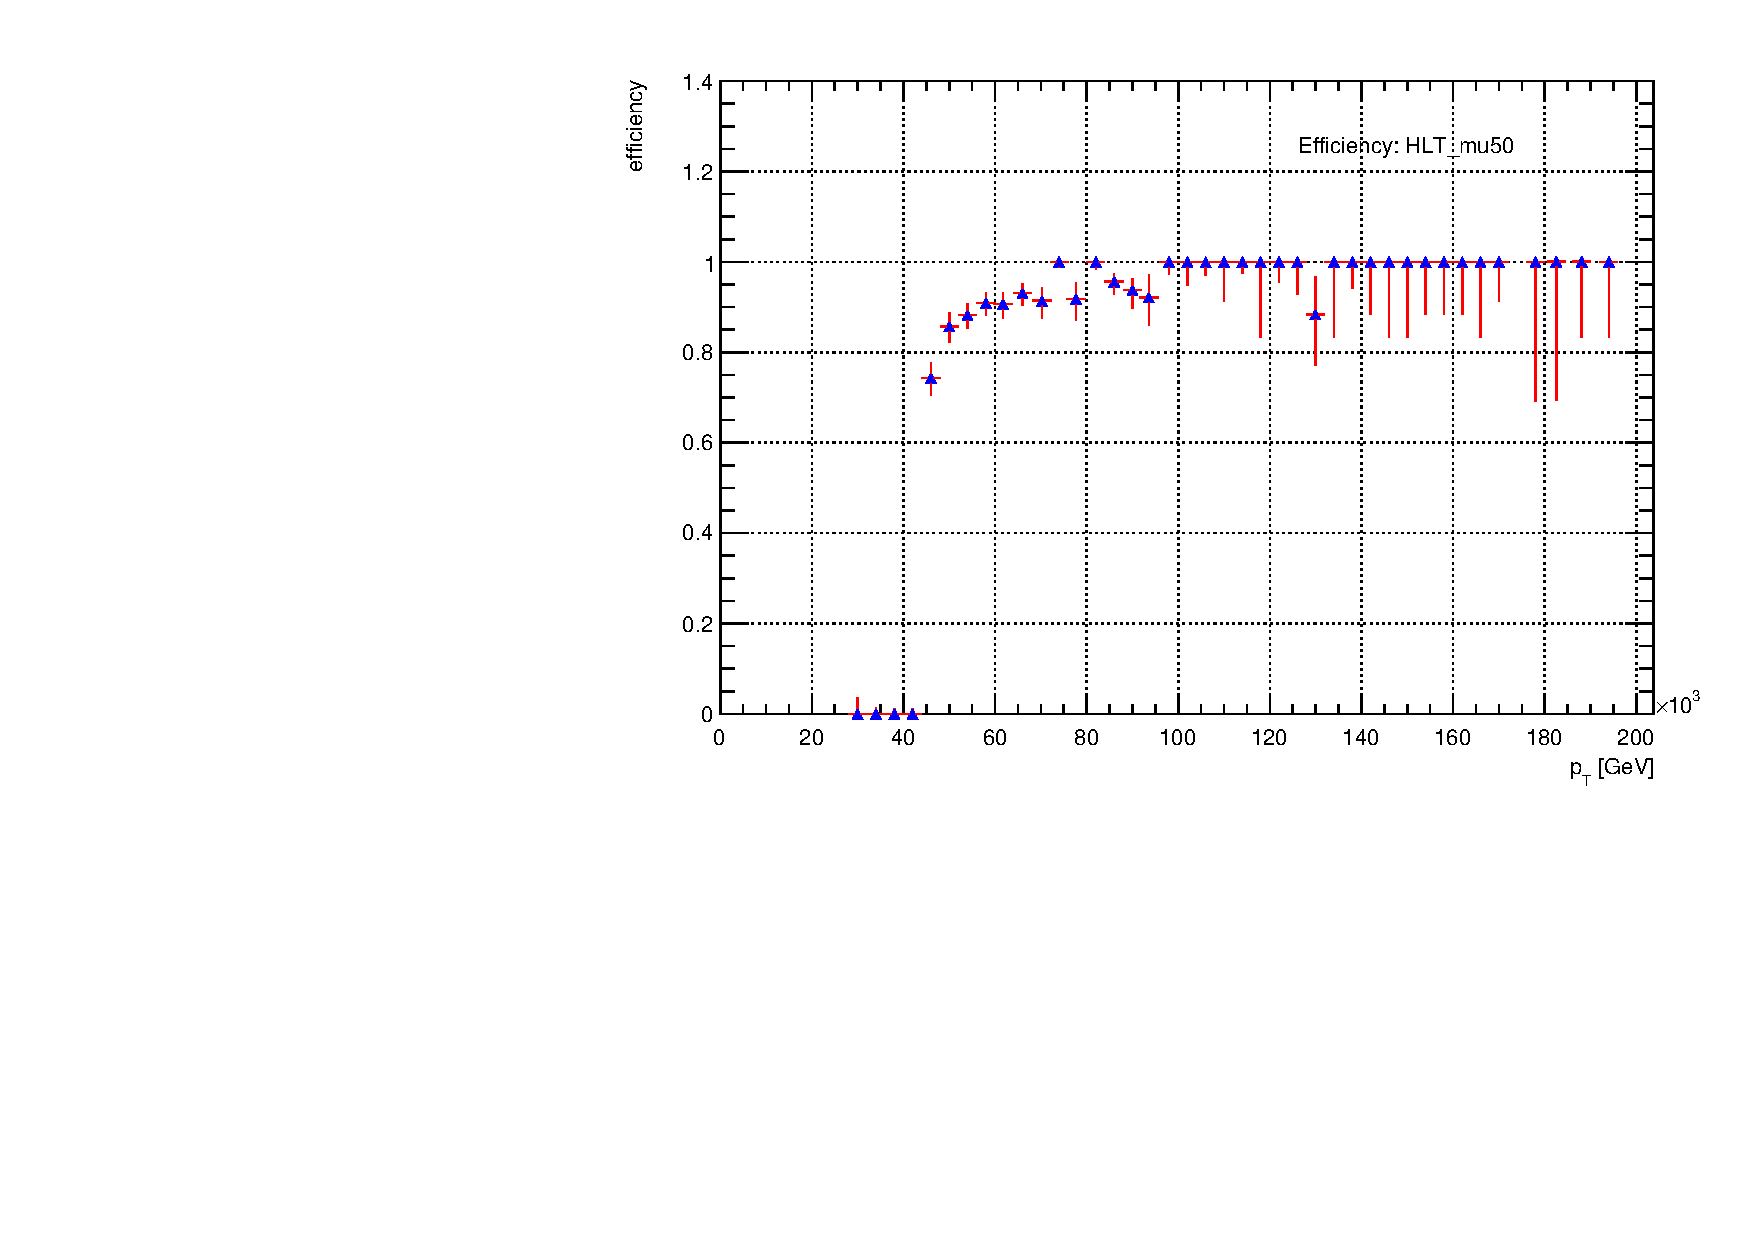
\includegraphics[width=0.48\textwidth]{TRIGGER/Eff_HLT_mu50}}
\subfigure{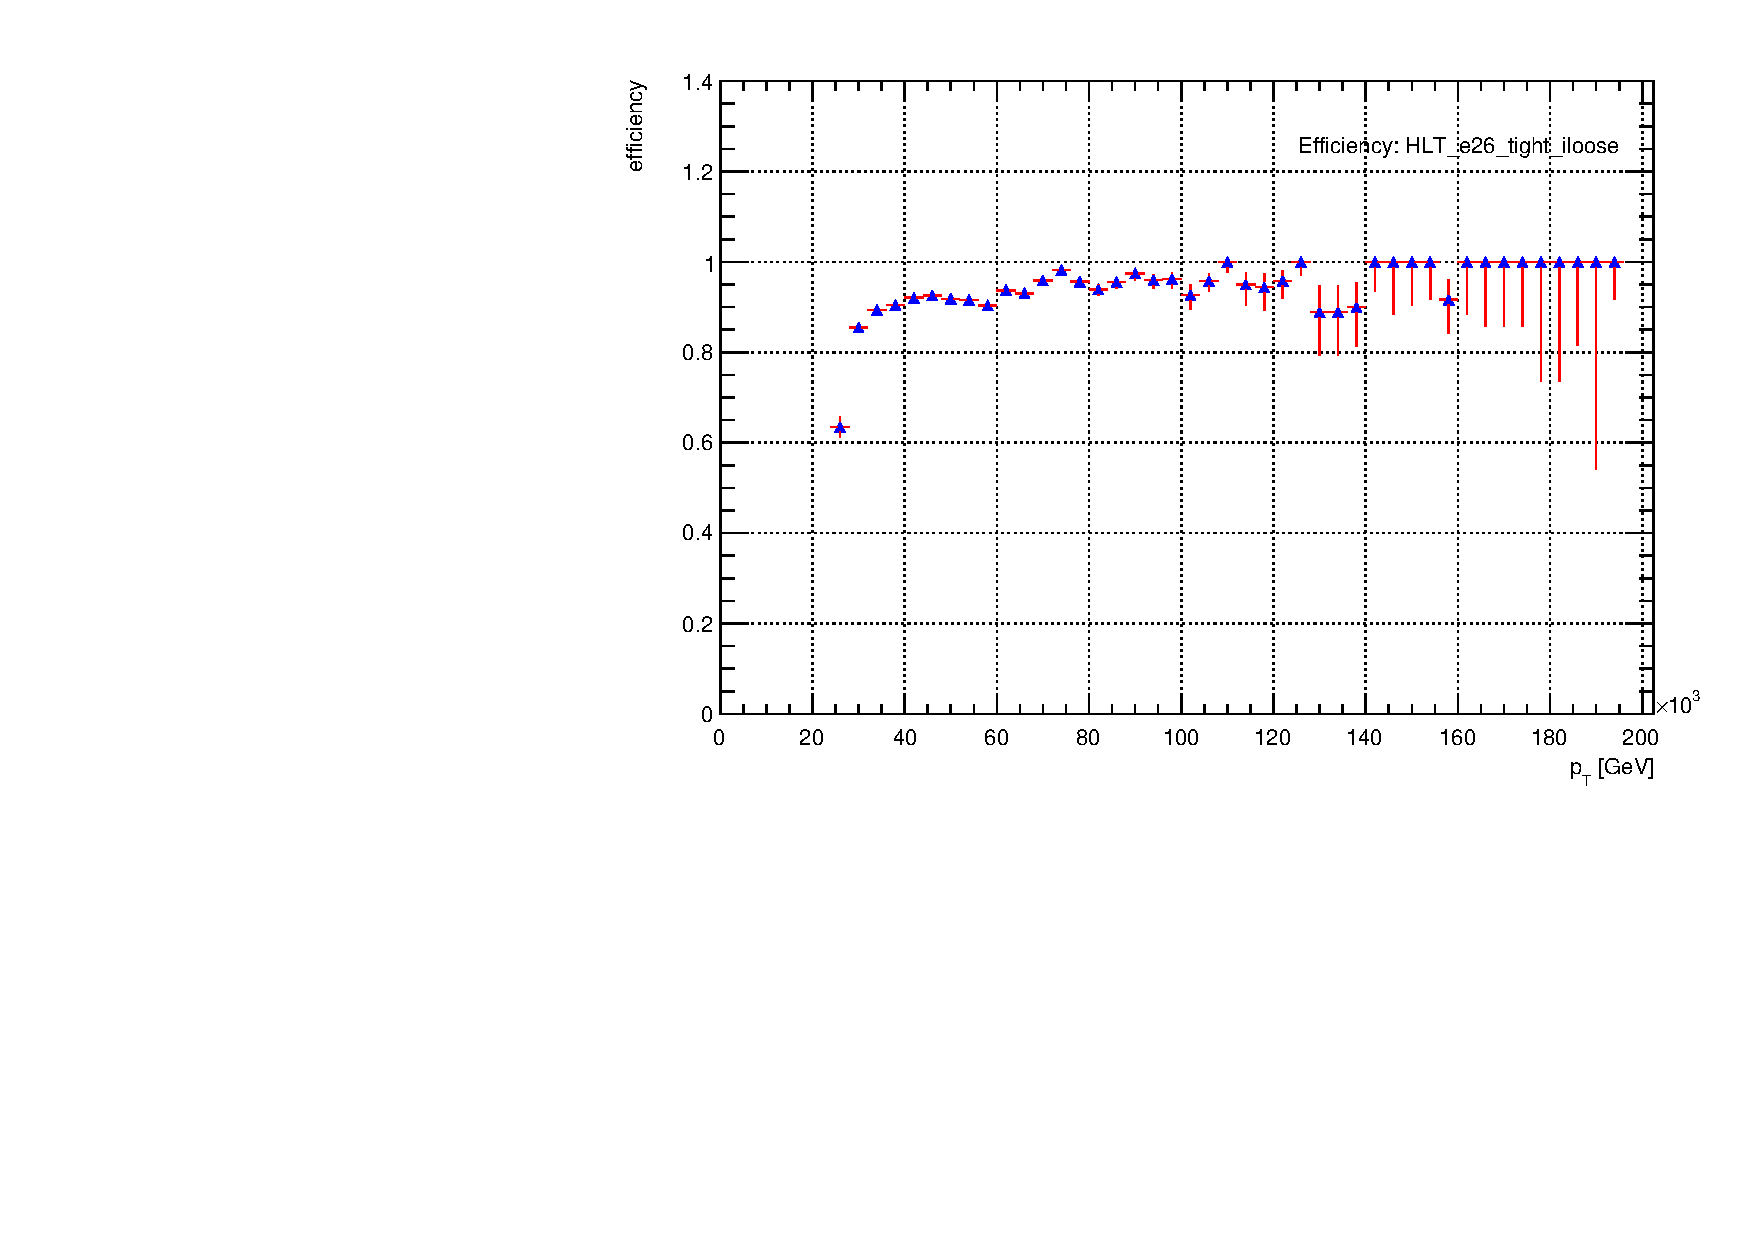
\includegraphics[width=0.48\textwidth]{TRIGGER/Eff_HLT_e26_tight_iloose}}
\caption{Trigger efficiencies for \texttt{HLT\_mu50} and \texttt{HLT\_e26\_tight\_iloose} versus \pt\ of the leading lepton. 
%The turn-on curves of the triggers are close to the expected threshold of the online efficiency. The efficiency on the trigger plateau is around 95\%.
}
\label{fig:eff_singlelepton}
\end{figure}

\begin{figure}[htb!]
\centering
\subfigure{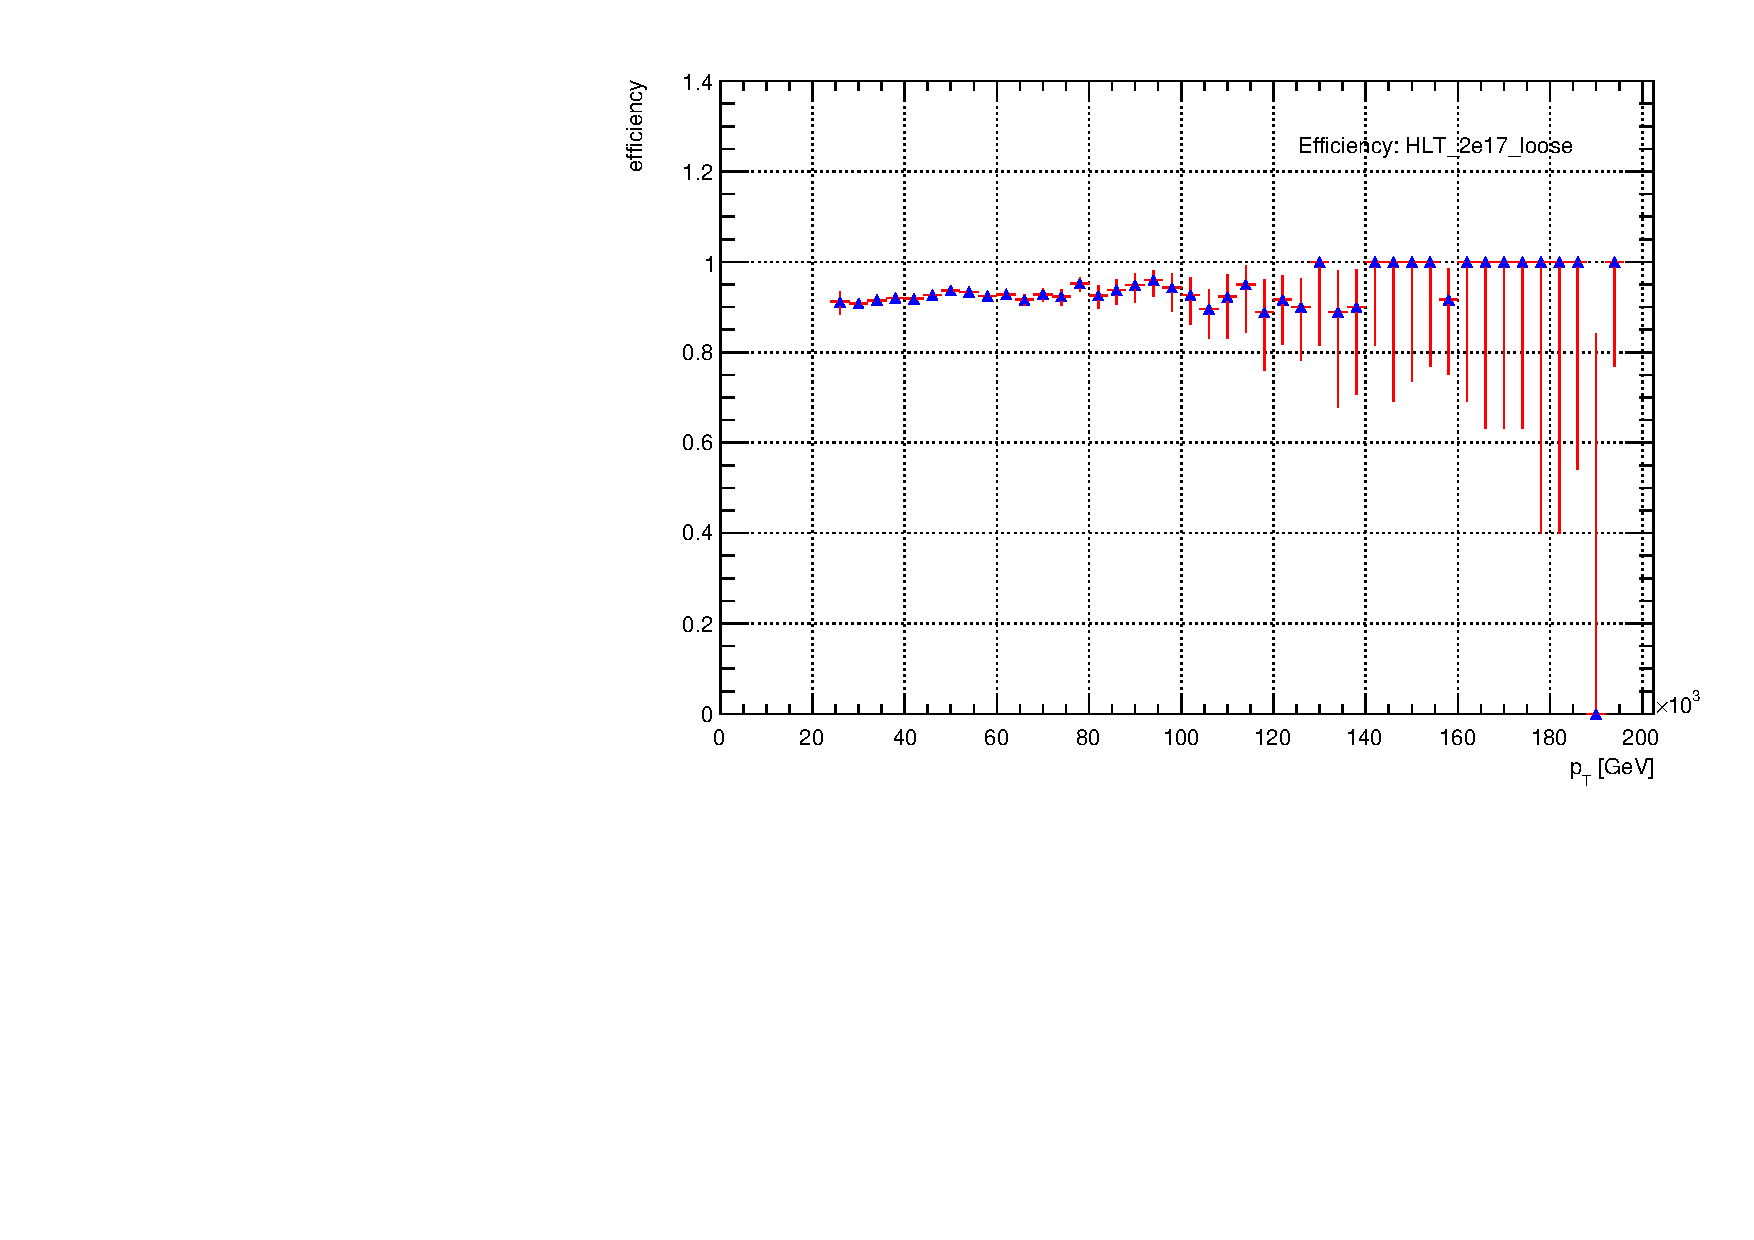
\includegraphics[width=0.48\textwidth]{TRIGGER/Eff_HLT_2e17_loose}}
\subfigure{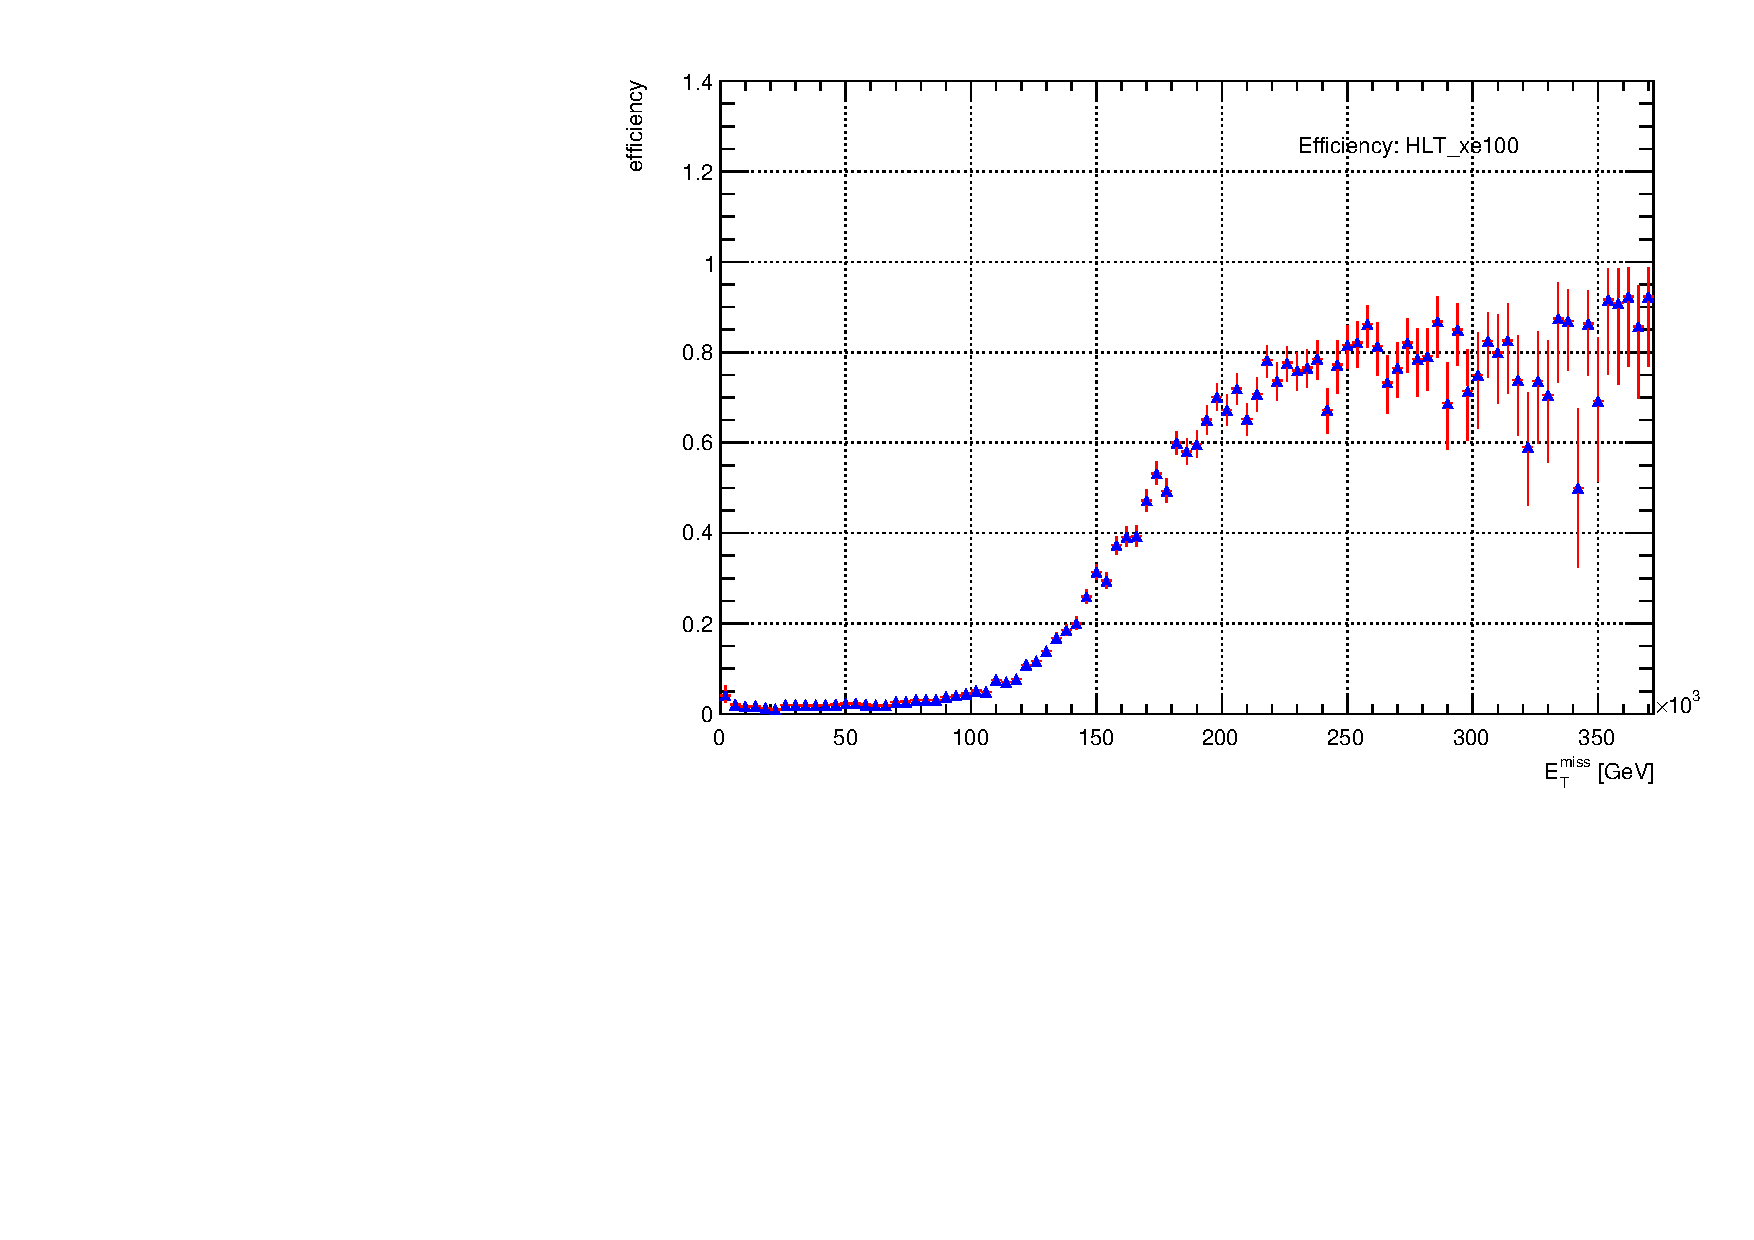
\includegraphics[width=0.48\textwidth]{TRIGGER/Eff_HLT_xe100}}
\caption{Trigger efficiencies for \texttt{HLT\_2e17\_loose} (left) and \texttt{HLT\_xe100} (right). The efficiency for the dilepton trigger is plotted against the \pt\ of the leading electron while the efficiency of the \met\ trigger is plotted against the corrected missing energy value. %Both triggers show the expected performance on the efficiency plateau. The dilepton trigger reaches an efficiency of around 90\%. For the \met\  trigger, the turn-on is slower. At the plateau it reaches also an efficiency of around 90\%.
}
\label{fig:eff_dilepton_met}
\end{figure}
